\subsubsection{1.1. Mô hình CNN baseline}
\indent\indent Trước khi đi vào xây dựng mô hình MGAT + FastKAN/MLP, đề tài đề xuất xây dựng và huấn luyện một kiến trúc CNN cơ sở (baseline) chỉ sử dụng dữ liệu hình ảnh. Mục tiêu của bước này là tạo ra một mốc tham chiếu (benchmark) để đánh giá sự cải thiện của các phương pháp đa phương thức được đề ra ở phía sau.\vspace{0.3cm}

\indent Kiến trúc của mô hình CNN baseline được minh họa tại \textbf{Hình \ref{fig:KTCNNBaseline}}, bao gồm các thành phần và cơ chế hoạt động như sau:
\begin{figure}[H]
    \centering
    \scalebox{0.5}{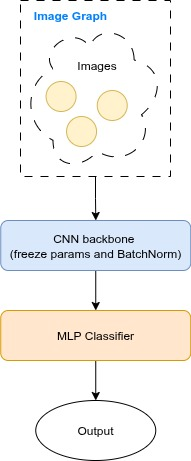
\includegraphics{images/part-02/chap-02/sec-01/CNNBaseline.jpg}}
    \vspace{0.3cm}
    \caption{Kiến trúc của mô hình CNN baseline}
    \label{fig:KTCNNBaseline}
\end{figure}

\textbf{Đầu vào (Image Graph):} Là dữ liệu ảnh đã được tiền xử lý bằng cách dùng các transforms từ các CNN backbone tương ứng.\vspace{0.3cm}

\textbf{Đầu ra (Output):} Kết quả dự đoán xác suất cho từng hình ảnh, sau đó tiền hành lấy trung bình cộng xác suất lại và cho ra kết quả phân lớp cuối cùng trên một mẫu đồ thị.\vspace{0.3cm}

\newpage
\textbf{Quy trình xử lý:}\vspace{-0.1cm}
\begin{itemize}[label={--}, itemsep=1pt]
    \item Trích xuất đặc trưng: Sáu kiến trúc CNN bao gồm ResNet18, RegNetX400MF, MobileNetV3 Large, MobileNetV3 Small, DenseNet121 và ShuffleNetV2 1.0x được sử dụng làm backbone trích xuất đặc trưng. Các mô hình này đều đã được huấn luyện trước trên tập dữ liệu ImageNet quy mô lớn. Điểm chính trong thiết kế CNN baseline nằm ở cơ chế đóng băng tham số (freezing), nhằm tận dụng các tri thức đã được học sẵn:\vspace{-0.1cm}
    \begin{itemize}[label={+}, itemsep=1pt]
        \item Freeze Parameters: Toàn bộ trọng số và bias của các lớp tích chập được giữ nguyên, không cập nhật trong quá trình lan truyền ngược. Điều này giúp bảo toàn khả năng nhận diện các đặc trưng cơ bản (cạnh, góc) mà mạng đã học được từ ImageNet.
        \item Freeze BatchNorm: Các lớp Batch Normalization cũng được chuyển sang chế độ đánh giá (eval mode), nghĩa là chúng sử dụng các giá trị trung bình (mean) và phương sai (variance) toàn cục đã học trước đó thay vì tính toán lại trên từng batch dữ liệu huấn luyện mới. Điều này đảm bảo tính ổn định của đặc trưng đầu ra.
        \end{itemize}
    \item Bộ phân lớp (MLP Classifier): Các đặc trưng sau khi đi qua backbone sẽ được đưa vào một mạng MLP. Đây là thành phần duy nhất có thể học được. Nhiệm vụ của MLP là học cách ánh xạ từ không gian đặc trưng của ImageNet sang không gian nhãn của ICH.
\end{itemize}